\documentclass{article}
\iffalse
This file is protected by Copyright. Please refer to the COPYRIGHT file
distributed with this source distribution.

This file is part of OpenCPI <http://www.opencpi.org>

OpenCPI is free software: you can redistribute it and/or modify it under the
terms of the GNU Lesser General Public License as published by the Free Software
Foundation, either version 3 of the License, or (at your option) any later
version.

OpenCPI is distributed in the hope that it will be useful, but WITHOUT ANY
WARRANTY; without even the implied warranty of MERCHANTABILITY or FITNESS FOR A
PARTICULAR PURPOSE. See the GNU Lesser General Public License for more details.

You should have received a copy of the GNU Lesser General Public License along
with this program. If not, see <http://www.gnu.org/licenses/>.
\fi

\author{} % Force author to be blank
%----------------------------------------------------------------------------------------
% Paper size, orientation and margins
%----------------------------------------------------------------------------------------
\usepackage{geometry}
\geometry{
	letterpaper,			% paper type
	portrait,				% text direction
	left=.75in,				% left margin
	top=.75in,				% top margin
	right=.75in,			% right margin
	bottom=.75in			% bottom margin
 }
%----------------------------------------------------------------------------------------
% Header/Footer
%----------------------------------------------------------------------------------------
\usepackage{fancyhdr} \pagestyle{fancy} % required for fancy headers
\renewcommand{\headrulewidth}{0.5pt}
\renewcommand{\footrulewidth}{0.5pt}
\rhead{\small{ANGRYVIPER Team}}
%----------------------------------------------------------------------------------------
% Appendix packages
%----------------------------------------------------------------------------------------
\usepackage[toc,page]{appendix}
%----------------------------------------------------------------------------------------
% Defined Commands & Renamed Commands
%----------------------------------------------------------------------------------------
\renewcommand{\contentsname}{Table of Contents}
\renewcommand{\listfigurename}{List of Figures}
\renewcommand{\listtablename}{List of Tables}
\newcommand{\todo}[1]{\textcolor{red}{TODO: #1}\PackageWarning{TODO:}{#1}} % To do notes
\newcommand{\code}[1]{\texttt{#1}} % For inline code snippet or command line
%----------------------------------------------------------------------------------------
% Various pacakges
%----------------------------------------------------------------------------------------
\usepackage{hyperref} % for linking urls and lists
\usepackage{graphicx} % for including pictures by file
\usepackage{listings} % for coding language styles
\usepackage{rotating} % for sideways table
\usepackage{pifont}   % for sideways table
\usepackage{pdflscape} % for landscape view
%----------------------------------------------------------------------------------------
% Table packages
%----------------------------------------------------------------------------------------
\usepackage{longtable} % for long possibly multi-page tables
\usepackage{tabularx} % c=center,l=left,r=right,X=fill
\usepackage{float}
\floatstyle{plaintop}
\usepackage[tableposition=top]{caption}
\newcolumntype{P}[1]{>{\centering\arraybackslash}p{#1}}
\newcolumntype{M}[1]{>{\centering\arraybackslash}m{#1}}
%----------------------------------------------------------------------------------------
% Block Diagram / FSM Drawings
%----------------------------------------------------------------------------------------
\usepackage{tikz}
\usetikzlibrary{shapes,arrows,fit,positioning}
\usetikzlibrary{automata} % used for the fsm
%----------------------------------------------------------------------------------------
% Colors Used
%----------------------------------------------------------------------------------------
\usepackage{colortbl}
\definecolor{blue}{rgb}{.7,.8,.9}
\definecolor{ceruleanblue}{rgb}{0.16, 0.32, 0.75}
\definecolor{drkgreen}{rgb}{0,0.6,0}
\definecolor{deepmagenta}{rgb}{0.8, 0.0, 0.8}
\definecolor{cyan}{rgb}{0.0,0.6,0.6}
\definecolor{maroon}{rgb}{0.5,0,0}
%----------------------------------------------------------------------------------------
% Update the docTitle and docVersion per document
%----------------------------------------------------------------------------------------
\def\docTitle{Component Data Sheet}
\def\docVersion{1.5}
%----------------------------------------------------------------------------------------
\date{Version \docVersion} % Force date to be blank and override date with version
\title{\docTitle}
\lhead{\small{\docTitle}}

\def\comp{e3xx\_mimo\_xcvr\_filter}
\def\proxy{e3xx\_mimo\_xcvr\_filter\_proxy}
\def\Comp{E3xx MIMO XCVR Filter and Proxy }
\graphicspath{ {figures/} }

\def\comp{e3xx\_mimo\_xcvr\_filter}
\edef\ecomp{e3xx_mimo_xcvr_filter}
\def\Comp{E3xx MIMO XCVR Filter}

\begin{document}

\section*{Summary - \Comp}
\begin{tabular}{|c|M{13.5cm}|}
	\hline
	\rowcolor{blue}
	                  &                                      \\
	\hline
	Names              & \comp, \proxy                        \\
	\hline
	Worker Types       & Device and Proxy \\
	\hline
	Version           & v\docVersion \\
	\hline
	Release Date      & 4/2019 \\
	\hline
	Component Library & ocpi.bsp.e310.cards   \\
	\hline
	Workers           & \comp.hdl, \proxy.rcc                \\
	\hline
	Tested Platforms  & E310 (Vivado only)                       \\
	\hline
\end{tabular}

\section*{Worker Implementation Details}
The \Comp workers are used to configure the analogue filter banks and frontend antenna switches for the Ettus E310 radio. A specific filter bank is selected based on the tuned LO frequency for the desired frontend channel. The frontend mode can be set directly to TX/Full Duplex, RX only, or off. Consult the tables in Reference \cite{usermanual}, the E310 User Manual, for full details on driver software operation.
\section*{Block Diagrams}
\subsection*{Top level}
\begin{figure}[ht]
	\centerline{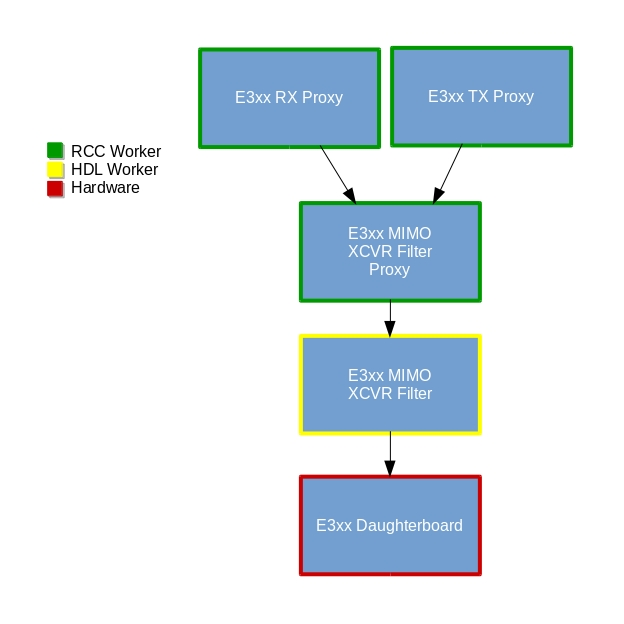
\includegraphics[scale=0.75]{e3xx_mimo_filter_top_level_diagram}}
	\caption{Top level block diagram of where the \Comp typically fit within a design}
	\label{fig:tb}
\end{figure}
\flushleft
Consult the E310 schematics in Reference \cite{schematics} for documentation of the hardware of the E3xx Daugherboard.
\section*{Source Dependencies}
\subsection*{\comp.hdl}
\begin{itemize}
	\item hdl/cards/\comp.hdl/\comp.vhd
\end{itemize}
\subsection*{\proxy.rcc}
\begin{itemize}
	\item hdl/cards/\proxy.rcc/\proxy.cc
\end{itemize}

\begin{landscape}
\section*{Component Spec Properties}
\subsection*{\comp.hdl}
	\begin{scriptsize}
		\begin{tabular}{|p{3.75cm}|p{1.25cm}|p{2cm}|p{2.75cm}|p{1.5cm}|p{1.5cm}|p{1cm}|p{6.23cm}|}
			\hline
            \rowcolor{blue}
            Name               & Type & SequenceLength & ArrayDimensions & Accessibility      & Valid Range & Default & Usage                                                                          \\
            \hline
            - & - & - & - & - & - & - & - \\
            \hline
        \end{tabular}
    \end{scriptsize}
\subsection*{\proxy.rcc}
	\begin{scriptsize}
		\begin{tabular}{|p{3.75cm}|p{1.25cm}|p{2cm}|p{2.75cm}|p{1.5cm}|p{1.5cm}|p{1cm}|p{6.23cm}|}
			\hline
            \rowcolor{blue}
            Name               & Type & SequenceLength & ArrayDimensions & Accessibility      & Valid Range & Default & Usage                                                                          \\
            \hline
            - & - & - & - & - & - & - & - \\
            \hline
        \end{tabular}
    \end{scriptsize}

\section*{Worker Properties}
\subsection*{\comp.hdl}
	\begin{scriptsize}
		\begin{tabular}{|p{2cm}|p{2.5cm}|p{1cm}|p{2cm}|p{2cm}|p{1.75cm}|p{2cm}|p{2cm}|p{5.29cm}|}
			\hline
			\rowcolor{blue}
			Scope        & Name                 & Type  & SequenceLength & ArrayDimensions & Accessibility & Valid Range & Default & Usage \\
			\hline
			Property     & \verb+TX_ENABLE1A+   & bool  & -              & -               & Writable      & Standard    & -       & Control Pin for TXA    \\
			\hline
			Property     & \verb+TX_ENABLE2A+   & bool  & -              & -               & Writable      & Standard    & -       & Control Pin for TXA    \\
			\hline
			Property     & \verb+TX_ENABLE1B+   & bool  & -              & -               & Writable      & Standard    & -       & Control Pin for TXB    \\
			\hline
			Property     & \verb+TX_ENABLE2B+   & bool  & -              & -               & Writable      & Standard    & -       & Control Pin for TXB    \\
			\hline
			Property     & \verb+VCTXRX1_V1+    & bool  & -              & -               & Writable      & Standard    & -       & Control Pin for TRXA Switch   \\
			\hline
			Property     & \verb+VCTXRX1_V2+    & bool  & -              & -               & Writable      & Standard    & -       & Control Pin for TRXA Switch   \\
			\hline
			Property     & \verb+VCTXRX2_V1+    & bool  & -              & -               & Writable      & Standard    & -       & Control Pin for TRXB Switch   \\
			\hline
			Property     & \verb+VCTXRX2_V2+    & bool  & -              & -               & Writable      & Standard    & -       & Control Pin for TRXB Switch   \\
			\hline
			Property     & \verb+VCRX1_V1+      & bool  & -              & -               & Writable      & Standard    & -       & Control Pin for RXA Switch   \\
			\hline
			Property     & \verb+VCRX1_V2+      & bool  & -              & -               & Writable      & Standard    & -       & Control Pin for RXA Switch   \\
			\hline
			Property     & \verb+VCRX2_V1+      & bool  & -              & -               & Writable      & Standard    & -       & Control Pin for RXB Switch   \\
			\hline
			Property     & \verb+VCRX2_V2+      & bool  & -              & -               & Writable      & Standard    & -       & Control Pin for RXB Switch   \\
			\hline
			Property     & \verb+TX_BANDSEL+    & uchar & -              & -               & Writable      & Standard    & -       & Control Pins for TX filter band selection   \\
			\hline
			Property     & \verb+RX1_BANDSEL+   & uchar & -              & -               & Writable      & Standard    & -       & Control Pins for RXA filter band selection   \\
			\hline
			Property     & \verb+RX1B_BANDSEL+  & uchar & -              & -               & Writable      & Standard    & -       & Control Pins for RXA filter band selection   \\
			\hline
			Property     & \verb+RX1C_BANDSEL+  & uchar & -              & -               & Writable      & Standard    & -       & Control Pins for RXA filter band selection   \\
			\hline
			Property     & \verb+RX2_BANDSEL+   & uchar & -              & -               & Writable      & Standard    & -       & Control Pins for RXB filter band selection   \\
			\hline
			Property     & \verb+RX2B_BANDSEL+  & uchar & -              & -               & Writable      & Standard    & -       & Control Pins for RXB filter band selection   \\
			\hline
			Property     & \verb+RX2C_BANDSEL+  & uchar & -              & -               & Writable      & Standard    & -       & Control Pins for RXB filter band selection   \\
			\hline
			Property     & \verb+LED_TXRX1_TX+  & bool  & -              & -               & Writable      & Standard    & -       & LED For TRXA in TX mode   \\
			\hline
			Property     & \verb+LED_TXRX1_RX+  & bool  & -              & -               & Writable      & Standard    & -       & LED For TRXA in RX mode   \\
			\hline
			Property     & \verb+LED_RX1_RX+    & bool  & -              & -               & Writable      & Standard    & -       & LED For RXA \\
			\hline
			Property     & \verb+LED_TXRX2_TX+  & bool  & -              & -               & Writable      & Standard    & -       & LED For TRXB in TX mode   \\
			\hline
			Property     & \verb+LED_TXRX2_RX+  & bool  & -              & -               & Writable      & Standard    & -       & LED For TRXB in RX mode   \\
			\hline
			Property     & \verb+LED_RX2_RX+    & bool  & -              & -               & Writable      & Standard    & -       & LED For RXB \\
			\hline
		\end{tabular}
	\end{scriptsize}
\subsection*{\proxy.rcc}
	\begin{scriptsize}
		\begin{tabular}{|p{1.5cm}|p{2.2cm}|p{2.5cm}|p{2.1cm}|p{2cm}|p{3.6cm}|p{1.5cm}|p{0.9cm}|p{4.75cm}|}
			\hline
			\rowcolor{blue}
			Scope        & Name                    & Type                             & SequenceLength & ArrayDimensions & Accessibility               & Valid Range & Default & Usage \\
			\hline
			Property     & \verb+rx_frequency_MHz+ & double                           & -              & -               & Writable,Readable,WriteSync & 0.7-6000    & -       & The property is written to notify the proxy worker to update the RX filter bank selection \\
			\hline
			Property     & \verb+tx_frequency_MHz+ & double                           & -              & -               & Writable,Readable,WriteSync & 0.7-6000    & -       & The property is written to notify the proxy worker to update the TX filter bank selection \\
			\hline
			Property     & \verb+trxa_mode+  & enum (tx,rx,off) & -              & -               & Writable,Readable,WriteSync & Standard    & -       & The property is written to instruct the proxy worker to configure the TRXA frontend antenna for the specified mode \\
			\hline
			Property     & \verb+rx2a_mode+  & enum (rx,off) & -              & -               & Writable,Readable,WriteSync & Standard    & -       & The property is written to instruct the proxy worker to configure the RX2A frontend antenna for the specified mode \\
			\hline
			Property     & \verb+trxb_mode+  & enum (tx,rx,off) & -              & -               & Writable,Readable,WriteSync & Standard    & -       & The property is written to instruct the proxy worker to configure the TRXB frontend antenna for the specified mode \\
			\hline
			Property     & \verb+rx2b_mode+  & enum (rx,off) & -              & -               & Writable,Readable,WriteSync & Standard    & -       & The property is written to instruct the proxy worker to configure the RX2B frontend antenna for the specified mode \\
			\hline
		\end{tabular}
	\end{scriptsize}

\section*{Component Ports}
\subsection*{\comp.hdl}
    \begin{scriptsize}
        \begin{tabular}{|p{2cm}|p{1.5cm}|p{4cm}|p{1.5cm}|p{1.5cm}|p{10.36cm}|}
        \hline
        \rowcolor{blue}
        Name & Producer & Protocol           & Optional & Advanced & Usage                  \\
        \hline
        -    & -        & -                  & -        & -        & - \\
        \hline
        \end{tabular}
	\end{scriptsize}
\subsection*{\proxy.hdl}
    \begin{scriptsize}
        \begin{tabular}{|p{2cm}|p{1.5cm}|p{4cm}|p{1.5cm}|p{1.5cm}|p{10.36cm}|}
        \hline
        \rowcolor{blue}
        Name & Producer & Protocol           & Optional & Advanced & Usage                  \\
        \hline
        -    & -        & -                  & -        & -        & - \\
        \hline
        \end{tabular}
	\end{scriptsize}

\section*{Signals}
\subsection*{\comp.hdl}
		\begin{scriptsize}
			\begin{tabular}{|c|c|c|c|p{2.6cm}|c|c|c|}
			\hline
			\rowcolor{blue}
			Name & Type  & Width & Description \\
			\hline
			TX\_ENABLE1A  & Out & 1     & Control Pin for TXA    \\
			\hline
			TX\_ENABLE2A  & Out & 1     & Control Pin for TXA    \\
			\hline
			TX\_ENABLE1B  & Out & 1     & Control Pin for TXB    \\
			\hline
			TX\_ENABLE2B  & Out & 1     & Control Pin for TXB    \\
			\hline
			VCTXRX1\_V1   & Out & 1     & Control Pin for TRXA Switch   \\
			\hline
			VCTXRX1\_V2   & Out & 1     & Control Pin for TRXA Switch   \\
			\hline
			VCTXRX2\_V1   & Out & 1     & Control Pin for TRXB Switch   \\
			\hline
			VCTXRX2\_V2   & Out & 1     & Control Pin for TRXB Switch   \\
			\hline
			VCRX1\_V1   & Out & 1     & Control Pin for RXA Switch   \\
			\hline
			VCRX1\_V2   & Out & 1     & Control Pin for RXA Switch   \\
			\hline
			VCRX2\_V1   & Out & 1     & Control Pin for RXB Switch   \\
			\hline
			VCRX2\_V2   & Out & 1     & Control Pin for RXB Switch   \\
			\hline
			TX\_BANDSEL   & Out & 3     & Control Pins for TX filter band selection   \\
			\hline
			RX1\_BANSEL     & Out & 3     & Control Pins for RXA filter band selection   \\
			\hline
			RX1B\_BANDSEL   & Out & 2     & Control Pins for RXA filter band selection   \\
			\hline
			RX1C\_BANDSEL   & Out & 2     & Control Pins for RXA filter band selection   \\
			\hline
			RX2\_BANSEL     & Out & 3     & Control Pins for RXB filter band selection   \\
			\hline
			RX2B\_BANDSEL   & Out & 2     & Control Pins for RXB filter band selection   \\
			\hline
			RX2C\_BANDSEL   & Out & 2     & Control Pins for RXB filter band selection   \\
			\hline
			LED\_TRX1\_TX     & Out & 1     & LED for TRXA in TX mode   \\
			\hline
			LED\_TRX1\_RX     & Out & 1     & LED for TRXA in RX mode   \\
			\hline
			LED\_RX1\_RX      & Out & 1     & LED for RXA \\
			\hline
			LED\_TRX2\_TX     & Out & 1     & LED for TRXB in TX mode   \\
			\hline
			LED\_TRX2\_RX     & Out & 1     & LED for TRXB in RX mode   \\
			\hline
			LED\_RX2\_RX      & Out & 1     & LED for RXB \\
			\hline
		\end{tabular}
	\end{scriptsize}
\end{landscape}

\section*{Control Timing and Signals}
The E3xx MIMO XCVR Filter device worker uses the standard Control Plane signals.

\begin{landscape}
\section*{Worker Configuration Parameters}
\subsubsection*{\comp.hdl}
\input{../../\ecomp.hdl/configurations.inc}
\section*{Performance and Resource Utilization}
\subsubsection*{\comp.hdl}
\input{../../\ecomp.hdl/utilization.inc}
\end{landscape}

\section*{Test and Verification}
No unit test for this component exists. However, a hardware-in-the-loop application (which is NOT a unit test) exists for testing purposes (see applications/e3xx\_mimo\_xcvr\_filter\_proxy\_test).

\begin{thebibliography}{2}
\bibitem{usermanual}
  E310 User Manual,
  \url{https://files.ettus.com/manual/page\_usrp\_e3x0.html}.
\bibitem{schematics}
  E310 Hardware Schematics,
  \url{https://files.ettus.com/schematics/e310/}.
\end{thebibliography}

\end{document}
